% THIS IS SIGPROC-SP.TEX - VERSION 3.1
% WORKS WITH V3.2SP OF ACM_PROC_ARTICLE-SP.CLS
% APRIL 2009
%
% It is an example file showing how to use the 'acm_proc_article-sp.cls' V3.2SP
% LaTeX2e document class file for Conference Proceedings submissions.
% ----------------------------------------------------------------------------------------------------------------
% This .tex file (and associated .cls V3.2SP) *DOES NOT* produce:
%       1) The Permission Statement
%       2) The Conference (location) Info information
%       3) The Copyright Line with ACM data
%       4) Page numbering
% ---------------------------------------------------------------------------------------------------------------
% It is an example which *does* use the .bib file (from which the .bbl file
% is produced).
% REMEMBER HOWEVER: After having produced the .bbl file,
% and prior to final submission,
% you need to 'insert'  your .bbl file into your source .tex file so as to provide
% ONE 'self-contained' source file.
%
% Questions regarding SIGS should be sent to
% Adrienne Griscti ---> griscti@acm.org
%
% Questions/suggestions regarding the guidelines, .tex and .cls files, etc. to
% Gerald Murray ---> murray@hq.acm.org
%
% For tracking purposes - this is V3.1SP - APRIL 2009

\documentclass{edm_template}

%\usepackage{amsmath} % might need this later..
%\usepackage{graphicx} % might need this later..
\usepackage{url,paralist,multirow}
\usepackage{color, colortbl}
\definecolor{Gray}{gray}{0.9}


\renewcommand{\arraystretch}{1.55}
\DeclareMathOperator*{\argmax}{arg\,max}
\newcommand{\mgr}[1]{\textsc{#1}}
\newcommand{\ftr}[1]{\textsc{#1}}

\newcommand{\comment}[1]{}

\begin{document}

\title{Student Profiling from Tutoring System Log Data: \\When do Multiple Graphical Representations Matter?}
%\subtitle{[Extended Abstract]
%\titlenote{A full version of this paper is available as
%\textit{Author's Guide to Preparing ACM SIG Proceedings Using
%\LaTeX$2_\epsilon$\ and BibTeX} at
%\texttt{www.acm.org/eaddress.htm}}}
%
% You need the command \numberofauthors to handle the 'placement
% and alignment' of the authors beneath the title.
%
% For aesthetic reasons, we recommend 'three authors at a time'
% i.e. three 'name/affiliation blocks' be placed beneath the title.
%
% NOTE: You are NOT restricted in how many 'rows' of
% "name/affiliations" may appear. We just ask that you restrict
% the number of 'columns' to three.
%
% Because of the available 'opening page real-estate'
% we ask you to refrain from putting more than six authors
% (two rows with three columns) beneath the article title.
% More than six makes the first-page appear very cluttered indeed.
%
% Use the \alignauthor commands to handle the names
% and affiliations for an 'aesthetic maximum' of six authors.
% Add names, affiliations, addresses for
% the seventh etc. author(s) as the argument for the
% \additionalauthors command.
% These 'additional authors' will be output/set for you
% without further effort on your part as the last section in
% the body of your article BEFORE References or any Appendices.

\numberofauthors{4} %  in this sample file, there are a *total*
% of EIGHT authors. SIX appear on the 'first-page' (for formatting
% reasons) and the remaining two appear in the \additionalauthors section.
%
\author{
% You can go ahead and credit any number of authors here,
% e.g. one 'row of three' or two rows (consisting of one row of three
% and a second row of one, two or three).
%
% The command \alignauthor (no curly braces needed) should
% precede each author name, affiliation/snail-mail address and
% e-mail address. Additionally, tag each line of
% affiliation/address with \affaddr, and tag the
% e-mail address with \email.
%
% 1st. author
% 2nd. author
\alignauthor 
Ryan Carlson\\
       \affaddr{Language Technologies Institute}\\
       \affaddr{Carnegie-Mellon University}\\
       \affaddr{Pittsburgh, PA 15213}\\
       \email{rcarlson@cs.cmu.edu}
% 3rd. author
\alignauthor 
Konstantin Genin\\
       \affaddr{Department of Philosophy}\\
       \affaddr{Carnegie-Mellon University}\\
       \affaddr{Pittsburgh, PA 15213}\\
       \email{kgenin@andrew.cmu.edu}
%\alignauthor
%Helga Caballero\\
%      \affaddr{School of Public and International Affairs}\\
%       \affaddr{University of Pittsburgh}\\
%      \affaddr{Pittsburgh, PA 15260}\\
%       \email{hec33@pitt.edu}
\and  % use '\and' if you need 'another row' of author names
% 4th. author
\alignauthor Martina Rau\\
       \affaddr{Human-Computer Interaction Institute}\\
       \affaddr{Carnegie-Mellon University}\\
       \affaddr{Pittsburgh, PA 15213}\\
       \email{marau@cs.cmu.edu}
% 5th. author
\alignauthor Richard Scheines\\
       \affaddr{Department of Philosophy}\\
       \affaddr{Carnegie-Mellon University}\\
       \affaddr{Pittsburgh, PA 15213}\\      
        \email{scheines@cmu.edu}
% 6th. author
%\alignauthor Clark Glymour\\
%       \affaddr{Department of Philosophy}\\
%       \affaddr{Carnegie-Mellon University}\\
%       \affaddr{Pittsburgh, PA 15213}\\      
%        \email{cg09@andrew.cmu.edu}
}

% There's nothing stopping you putting the seventh, eighth, etc.
% author on the opening page (as the 'third row') but we ask,
% for aesthetic reasons that you place these 'additional authors'
% in the \additional authors block, viz.
%\additionalauthors{Additional authors: John Smith (The Th{\o}rv{\"a}ld Group,
%email: {\texttt{jsmith@affiliation.org}}) and Julius P.~Kumquat
%(The Kumquat Consortium, email: {\texttt{jpkumquat@consortium.net}}).}
%\date{30 July 1999}
% Just remember to make sure that the TOTAL number of authors
% is the number that will appear on the first page PLUS the
% number that will appear in the \additionalauthors section.

\maketitle
\begin{abstract}
We analyze log-data generated by an experiment with Mathtutor, an intelligent tutoring system for fractions.  The experiment compares the educational effectiveness of instruction with single and multiple graphical representations. We extract the error-making and hint-seeking behaviors of each student to characterize their learning strategy. Using an expectation-maximization approach, we cluster the students by their learning strategy. We find that a) experimental condition and learning outcome are clearly associated b) experimental condition and learning strategy are not, and c) almost all of the association between experimental condition and learning outcome is found among students implementing just one of the learning strategies we identify. This class of students is characterized by relatively high error-rates as well as a marked reluctance to seek help. They also show the greatest educational gains from instruction with multiple rather than single representations.The behaviors that characterize this group illuminate the mechanism underlying the effectiveness of multiple representations and suggest strategies for tailoring instruction to individual students. Our methodology can be implemented in an on-line tutoring system to dynamically tailor individualized instruction.

\end{abstract}

%% A category with the (minimum) three required fields
%\category{H.4}{Information Systems Applications}{Miscellaneous}
%%A category including the fourth, optional field follows...
%\category{D.2.8}{Software Engineering}{Metrics}[complexity measures, performance measures]
%
%\terms{Theory}

%\keywords{ACM proceedings, \LaTeX, text tagging} % NOT required for Proceedings

\section{Introduction}
\label{sec:introduction}

Multiple Graphical Representations (MGRs) are used extensively in middle-school fraction instruction.  Fractions can be alternately presented as pie and rectangle graphs, number lines, or discrete sets of objects. The educational psychology literature suggests that MGRs support transfer because requiring students to translate between representations makes them more likely to create deep knowledge structures \cite{Ambrose2010}. Nevertheless, the experimental results are somewhat ambiguous \cite{Ainsworth1999} and the mechanisms through which multiple representations influence student achievement are not well understood \cite{Ainsworth2006}. 

Because user interaction with intelligent tutoring systems (ITSs) generates large amounts of behavioral and outcome data, these systems are well-suited for conducting experiments on the effect of MGRs on learning outcomes \cite{Newell1981}. Machine learning methods can be profitably applied to identify the kinds of students that are successful and the factors mediating their success. We are particularly concerned with designing adaptive educational environments that support effective learning behaviors. This may involve encouraging students to reflect on the material with self-explanation prompts \cite{Rau2009} or detecting ineffective strategies and implementing interventions on-the-fly. Work in the latter area ranges from detecting abuse of the ITS hint system and other ``gaming'' behaviors \cite{Baker2009,Baker2009b} to providing spontaneous help to students lacking the meta-cognitive skills to know when they could use a hint \cite{Aleven2000,Aleven2003,Aleven2006}.

Prior work conducted on middle-school students working with a Cognitive Tutor for fractions found that multiple representations, in conjunction with self-explanation prompts, contribute to improved learning outcomes \cite{Rau2009}. Subsequent studies examining error-rate, hint-use and time-spent in tutor's log failed to identify variables that mediate the effectiveness of multiple representations \cite{Rau2012}. The mechanisms by which multiple representations improve learning outcomes remain poorly understood.

We conjecture that previous efforts to identify mediating factors were frustrated by heterogeneity in the problem-solving habits and behaviors of the student population under investigation. Using a mixture modeling technique, we cluster students by the patterns of interaction with the tutor in the log-data that characterize their learning strategy. Clustering based on student characteristics has proved successful in grouping students into meaningful subpopulations across both collaborative \cite{Perera2009} and individual \cite{Merceron2005} educational environments. 

Four strategic profiles emerge from our analysis, each with a natural interpretation. Two of the profiles are characterized by a low propensity to seek help from the tutor. In one of these the students are simply confident: they make few errors, solicit little help and don't seem to need any. In the other they are stubborn: they make a relatively large number of mistakes but make little use of the support mechanisms the tutor provides. A third class is highly interactive: they make many mistakes, seek assistance readily and frequently exhaust the hints available in a given problem. Students in the fourth class occupy a middle ground between the interactive and the stubborn: they make an average number of mistakes and will eventually seek help when they are having trouble.

We proceed to explore how the experimental conditions affect post-test outcomes. Confirming previous results, we find that students in the multiple-representation condition had greater learning gains than those in the sing-representation condition. Multiple representations seem to have a robust and positive effect on long-term knowledge consolidation. We then explore the effect of multiple representations in the sub-populations defined by each strategic profile. We first establish independence between learning strategy and experimental condition. This suggests that we are detecting pre-existing learner profiles, rather than artifacts of the experimental setup. Most interestingly, we discover that learning gains from MGRs depend heavily on cluster membership. Students exhibiting a ``stubborn'' profile profited substantially from instruction with multiple rather than single representations. For the remaining students, experimental condition and learning gain were independent. We conjecture that ``stubborn'' students lack the meta-cognitive skills to judge when their learning strategies are failing. These students are the most sensitive to pedagogical decisions because they are the least equipped to structure and manage their own learning. 

Section \ref{sec:experiment} of what follows describes the initial experiment and elaborates on the differences between the representational conditions. We describe our feature extraction process and modeling decisions in Section \ref{sec:method}. Section \ref{sec:results} summarizes the results of the model estimation and statistical analysis of the effects of multiple representations at the population and sub-population levels. We  suggest profitable future directions in Section \ref{sec:conclusion}.

\section{Experiment}
\label{sec:experiment}

In the Spring of 2010, Rau conducted an experiment wherein 290 $4^\text{th}$ and $5^\text{th}$ grade students worked with an interactive fractions tutor for about 5 hours of their mathematics instruction. Students were randomly assigned to one of five experimental conditions, which varied by the frequency with which students would be presented with a new fraction representation. Students in the \mgr{Single} representation condition worked exclusively with either a number line, a circle or a rectangle. Students in the \mgr{Fully Interleaved} condition would see a different representation with every new problem. Students in the intermediate conditions would go longer before they were presented with a different representation.   
\begin{figure}[htbp]
\centering
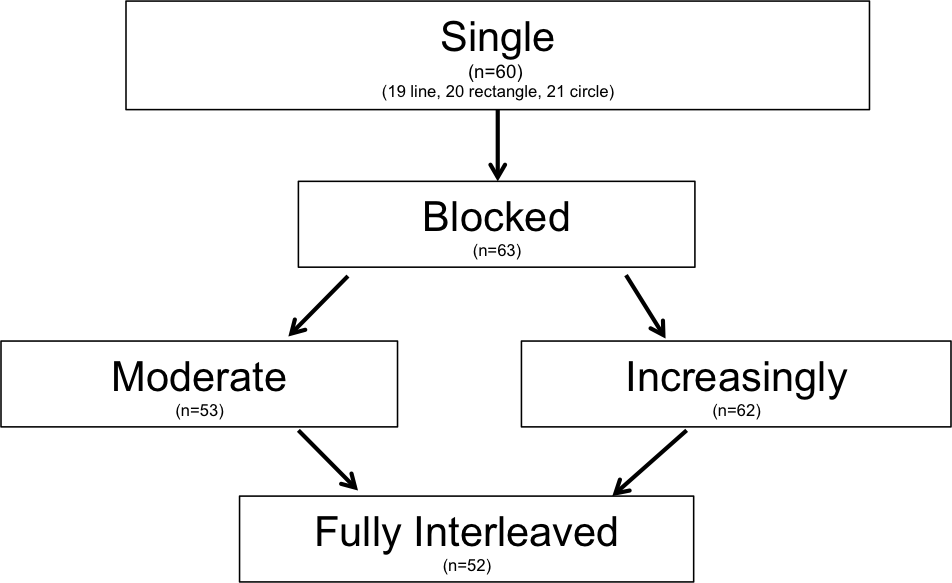
\includegraphics[scale=.4]{conditionGraph.png}\\
\caption{A partial ordering of experimental conditions by the frequency with which a new representation is presented. }
\label{fig:condition-graph}
\end{figure}

When interacting with different graphical representations of fractions, students were able to drag-and-drop slices of a pie graph, for example, into separate areas. They were also able to experiment with changing the number of subdivisions in each graphical representation. Students received a pre-test on the day before they began working with the tutor and an immediate post-test on the day after they finished. Students also took a delayed post-test a week after the first. Previous investigation found that students in the multiple representation conditions significantly outperformed students in the single representation condition on the delayed post-test \cite{Rau2012,Rau2012b}. 

%\section{Related Work}
%\label{sec:related-work}

%Latent Class Analysis and other clustering tools have commonly been used to analyze educational data. LSA can be used either for explanatory or confirmatory purposes. An application of clustering for educational data is presented in \cite{Merceron2005}, where students were clustered by types of mistakes. The authors suggested that identifying the different types of learners could help teachers apply remedial methods. Similarly, \cite{Perera2009} applied clustering techniques to group teams of students by the amount of work they performed. With LSA techniques they were able to reduce seven groups to three clusters. \cite{Maas2008} provided a comparative analysis of simulated data for Rule Assessment Methodology and LSA. They found five classes with conditional probabilities close to 0.95. They also found that the five classes worked better with RAM than the previous class definitions. Finally, \cite{Su2006} proposed a four-phase learning portfolio mining (LPM) approach, which uses sequential pattern mining, clustering and decision tree creation to find features from the portfolio and predict which group a new learner belongs to. Additional techniques used in educational data mining can be found in \cite{Romero2007}.
 
\section{Method}
\label{sec:method}

We proceed in three stages: (1) we extract features characterizing error and hint-seeking behavior from the data logs, (2) we transform the longitudinal log data into a cross-sectional form, with one observation per student, and (3) we estimate a mixture model to identify sub-populations of students, using AIC and BIC to select the number of classes. 

Once we have clustered our students by their learning strategy, we investigate the interaction between the strategies and the experimental conditions. We construct a contingency table binning the experimental conditions into the clusters estimated by the mixture model. We then run a Chi-squared test for independence between experimental condition and learning strategy. Chi-squared tests are also run to investigate dependence between pre-test outcome and strategy, strategy and post-test outcome and the conditional dependence of outcome and experimental condition, given a strategy profile.

\subsection{Extracting Features}
The Cognitive Tutor captures a detailed log of each student's interactions with the tutor. It stores a time series of correct and incorrect answers, hint requests, interface selections and durations between interactions. Previous analysis \cite{Rau2012} extracted the average number of errors made per step, the average number of hints requested per step, and the average time spent per step from the log data. Similarly, we include the average number of hints requested (\ftr{HintsRequested}) and number of errors (\ftr{NumErrors}) made per \emph{problem} by each student. We also extract the average number of bottom-out hints (\ftr{NumBOH}) per student per problem -- this is the average number of times a student exhausts the available hints in a given problem. We also note that it is not always the average of these features that best characterizes a student. For example, examination of the distribution of hints requested per step across experimental condition, shows a telling picture.
\begin{figure*}[t!]
\centering
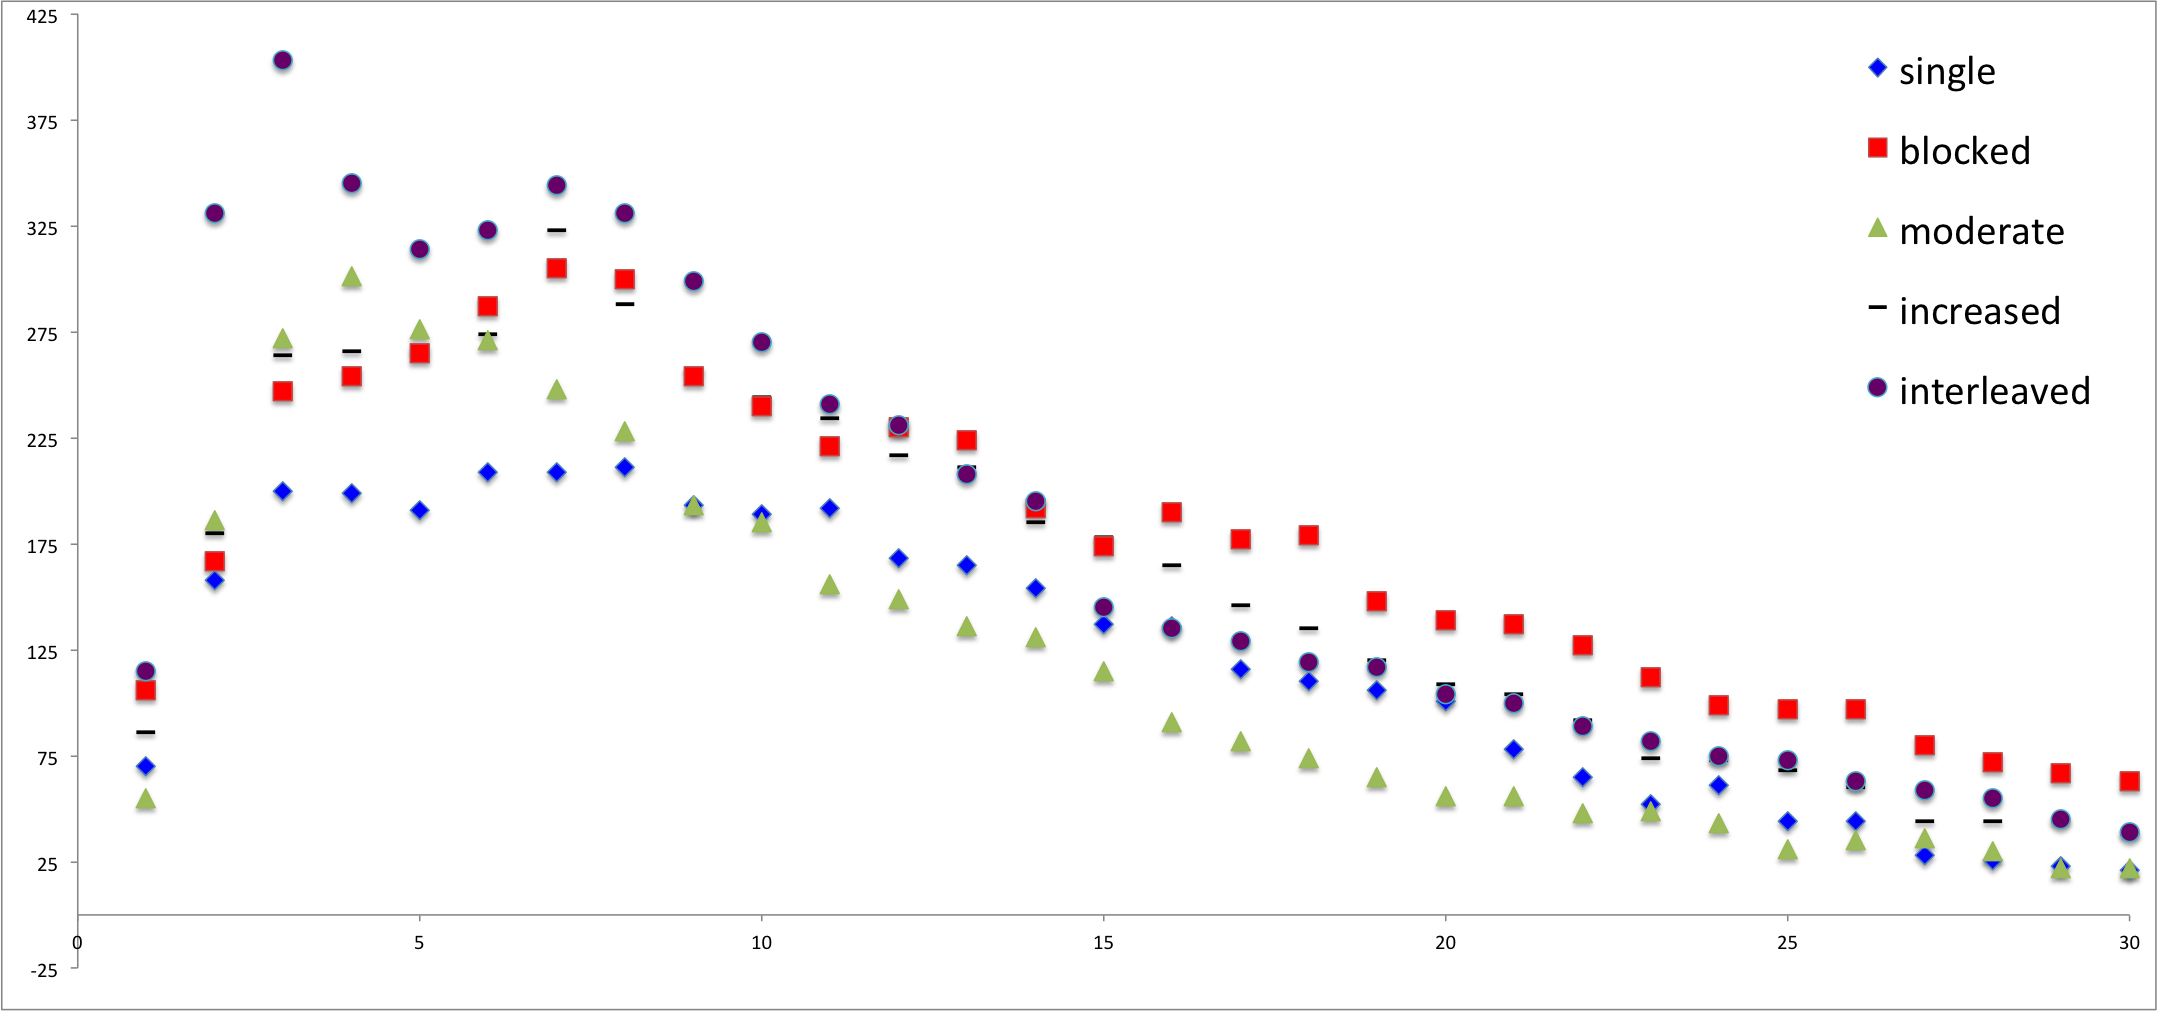
\includegraphics[scale=.48]{hintsByStep2.png}\\
\caption{The $x$-axis represents the $n_{th}$ interaction with the tutor across all problems. The $y$-axis is the total number of hints requested at the $n_{th}$ step.  }
\label{fig:condition-graph}
\end{figure*}

Note that students who received only one representation start out requesting the fewest hints, but students in the moderate condition eventually need fewer  (Figure \ref{fig:condition-graph}). Such considerations motivated our interest in the temporal distribution of hint behavior at the student level. We fit geometric distributions to the number of steps taken before the first hint request (\ftr{FirstHintGeometric}) and to the number of errors before the first hint (\ftr{StubbornGeometric}). The estimated parameter is used to characterize the student's hint-seeking propensity in general and hint-seeking propensity when faced with adversity. For example, students in the first quintile of \ftr{StubbornGeometric} seek help soon after making a mistake, whereas students in the fifth quintile don't change their hint-seeking behavior even after making a large number of errors. Students in the first quintile of \ftr{FirstHintGeometric} are likely to request hints early in a problem, whereas students in the fifth quintile are unlikely to request hints at any point.
\begin{table*}[htbp]
\caption{Summary Statistics for Variables Used in Clustering}
\begin{center}
\begin{tabular}{| l || c | c || c | c | c || c | c | c | c | c |}
\hline
&mean& sd&median&min&max&20\%&40\%&60\%&	80\%&100\%\\ \hline \hline
\ftr{HintsRequested}&0.78&1.27&0.34&0&11.22&0.06&0.19&0.5&1.31&11.22\\ \hline
\ftr{NumErrors}&2.21&1.27&1.92&0.34&8.39&1.15&1.7&2.18&3.19&8.39\\ \hline 
\ftr{FirstHintGeometric}&0.35&0.27&0.27&0.04&1&0.13&0.2&0.33&0.57&1\\ \hline
\ftr{Stubborn Geometric}&0.36&0.21&0.31&0.07&1&0.19&0.27&0.38&0.47&1\\ \hline
\ftr{NumBOH}&0.04&0.08&0&0&0.62&0&0&0.01&0.05&0.63\\ \hline
 \end{tabular}
\end{center}
\label{tab:sumstats}
\end{table*}

\subsection{Expectation-Maximization Clustering}
\label{sec:EM-clust}

Expectation-Maximization (EM) clustering is a modeling technique that determines subtypes based on multinomial distributions. We use the model to categorize students into subpopulations using discretized versions of the features described above. Table \ref{tab:sumstats} shows summary statistics and cut-off points for the extracted features. The model maps a set of observed categorical variables onto a set of inferred classes. 

We note that the categorical nature of the model has the potential to add some noise, since we must select numeric cutoffs to transform our variables into nominals. However, categorical models can offer greater interpretability by allowing us to organize our data into a small set of variables, which forms the basis for categorizing students into a small set of meaningful homogenous groups. Furthermore, it is not unreasonable to suspect that our variables are in some sense ``truly'' categorical \cite[pp8--9]{Collins2009}. 

%The formal representation of LSA begins with $j = 1 \ldots J$ observed variables, where each such variable $j$ has a set of response variables $r_{j} = 1,\ldots,R_{j}$. Each student has a distinct response pattern $y = (r_{1},\ldots,r_{j})$.

%Now we need to consider the latent classes. Let $L$ be a latent variable with latent classes $c~=~1,\ldots,C$. Furthermore, let $\gamma_{c}$ be the probability of membership in class $c$. Note that latent classes are exhaustive and mutually exclusive, so each student is a member of exactly one latent class. We also need to define the item-response probability $\rho_{j,r_{j}|c}$, which is the probability of response $r_{j}$ to observed variable $j$, conditional on membership in latent class $c$. Each student provides exactly one response alternative to variable $j$. Given these constraints, note that
%\[ \sum_{c=1}^{C} \gamma_{c} = 1,\quad \sum_{r_{j}=1}^{R_{j}} \rho_{j,r_{j}|c} = 1. \] 

%Now that we have defined key variables, we can define the probability of observing a particular response vector based on the $\gamma$'s and $\rho$'s:
%\begin{align}
%P(Y = y) = \sum_{c=1}^{C} \gamma_{c} \prod_{j=1}^{J} \prod_{r_{j}=1}^{R_{j}} \rho_{j,r_{j}|c}^{I(y_{j} = r_{j})}
%\label{eqn:LSA-final}
%\end{align}
%where the indicator function $I(y_{j} = r_{j})$ equals 1 when the response variable $j = r_{j}$. The parameters $\gamma_{c}$ and $\rho_{j,r_{j}|c}$ are estimated by EM. Since EM is sensitive to starting probabilities, we pick the maximum likelihood over twenty-five runs. LSA is very similar to other EM-based algorithms. In fact, LSA is an application of multivariate mixture estimation using categorical variables with an additional local independence assumption, meaning that the observed variables are independent of each other conditional on the latent variable. This is a simplifying assumption similar to the one made in Naive Bayes classification models; without it Equation \ref{eqn:LSA-final} would have to be much more complicated. There is some work on relaxing this independence assumption \cite{Hagenaars1988,Garrett2004}. For more details on the formalism and its applications, see \cite{Collins2009}. To run latent class analysis, we used \texttt{poLSA}, a freely available R package\footnote{\url{http://userwww.service.emory.edu/~dlinzer/poLSA/}}.

Note that unlike some common clustering algorithms (e.g., k-means), EM produces ``fuzzy'' clusters (i.e., probability distributions over features for each class). We use these probability distributions in our qualitative discussion about the subpopulations (Section \ref{sec:exploring-classes}), however we ultimately need to identify each student's most likely class. For each student $s$ and class $c$ we calculate
\begin{align}
\argmax_{c} P(S = s \;|\; L = c)
%\argmax_{c} P(Y = y \;|\; L = c) = \argmax_{c} \gamma_{c} \prod_{j=1}^{J} \prod_{r_{j}=1}^{R_{j}} \rho_{j,r_{j}|c}^{I(y_{j} = r_{j})}
\label{eqn:LCA-argmax}
\end{align}
where the probabilities are determined by the EM algorithm.

Note that still need to fix $C$, the number of classes. We use two complexity-penalized log-likelihood scores to select an appropriate $C$: Akaike information criterion (AIC) and Bayesian information criterion (BIC). Plotting these statistics as we increment the number of classes, we look for a ``knee'' where both statistics either bottom-out or level off to identify the optimal value of $C$. To run analysis, we used \texttt{poLCA}, a freely available R package\footnote{\url{http://userwww.service.emory.edu/~dlinzer/poLCA/}}.

\section{Results}
\label{sec:results}

In the sections that follow we analyze the results of our clustering algorithm. We describe the classes that were generated and characterize the students in each class. We then consider the relationships between our variables of interest: 
\begin{inparaenum}[\itshape (a)]
\item adjusted delayed post-test score,
\item experimental condition (the graphical representation condition), and
\item cluster membership.
\end{inparaenum}
Specifically, we run a series of Chi-squared tests for independence to determine how each variable interacts with the others, commenting on the importance of each comparison. Finally, we explore the stability of these classes, which bears on whether future systems could categorize student strategy profiles in real time.

\subsection{Exploring the Learning Strategies}
\label{sec:exploring-classes}

Figure \ref{fig:LCa-test-statistics} shows the parameter selection process described in Section \ref{sec:EM-clust}. Note that we chose to model four classes because BIC bottoms out and AIC levels off at that point.

\begin{figure}[htbp]
%\centering
\includegraphics[scale=0.4]{LCa-stats-plot.png}
\caption{AIC and BIC over increasing number of clusters. BIC bottoms out and AIC levels off at four clusters, so we conclude that four clusters best fits the data.}
\label{fig:LCa-test-statistics}
\end{figure}

After selecting the appropriate $C$ parameter, we extract membership probabilities for the individual students. Given a strategy profile, we know the probability distribution over each feature, and use Equation \ref{eqn:LCA-argmax} to identify the most likely profile for each student.

The feature distributions over each profile are represented graphically in Figure \ref{fig:LCa-class-viz}. Note that each feature is listed along the horizontal $x$-axis, the value each variable takes is along the front-to-back $y$-axis, and the probability that the feature takes that value is given along the vertical $z$-axis. For example, consider the \ftr{HintsRequested} feature (average hints requested per problem) in Class 2. In that class, with high probability, students requested many hints (i.e., the highest categorical value for hints) per problem on average. As another example, students in Class 1 are more likely to make a moderate number of errors, though other error levels also occur with nontrivial probabilities. Note that lower values of \ftr{FirstHintGeometric} and \ftr{StubbornGeometric} indicate a steep geometric slope, corresponding to a higher hint-seeking propensity and stubbornness, respectively.

How do we interpret cluster membership? Students in Class 1 are ``Moderate'', they ask for a moderate number of hints, make a moderate number of errors, and are moderately responsive to the interface. Students in Class 2 are ``Interactive'', they make a lot of errors, but respond by requesting many hints. These students are proactive in asking for help and are not shy about using the resources the cognitive tutor makes available. Students in Class 3 are ``Confident'', they don't ask for hints, but they don't seem to need them (since they make few errors). Finally, we call students in Class 4 ``Stubborn'' because they are fairly mixed in error-profile but they don't respond to mistakes with hint-requests. These students are not using all the resources that the cognitive tutor makes available.

\begin{figure*}[t]
\centering
\includegraphics[scale=0.5]{LCa-class-viz.png}
\caption{Visualization of feature distributions for each learning profile. The left-to-right $x$-axis identifies each feature, the front-to-back $y$-axis identifies which value that feature takes, and the top-to-bottom $z$-axis describes the probability that the feature takes the value. Thus, given a feature and a class, the $z$-axis also describes the probability distribution over that feature in that class.}
\label{fig:LCa-class-viz}
\end{figure*}


\subsection{Condition and Outcome} 
We use normalized learning gain at the delayed post-test as our measure of student improvement. 
\begin{center}
\textsc{Adjusted Post-Test} = \scalebox{1.2}{$\frac{\text{\textsc{PostTest}} - \text{\textsc{PreTest}}}{1-\text{\textsc{PreTest}}}$}
\end{center}

We then construct terciles of the Adjusted Delayed Post-Test Score and run a Chi-squared test for independence of outcome from experimental condition. Confirming previous results, we reject independence at a $p$-value of .024 (see Table \ref{tab:exp-and-score}). As expected, students in the multiple representation conditions were more likely to be in the second or third tercile of adjusted delayed post-test score, whereas students in the single representation condition were more likely to be in the first.

\begin{table}[hbtp]

\centering
\begin{tabular}{|l || c | c | c |}
\hline
&33\%&66\%&99\%\\ \hline \hline
  \textbf{blocked}  &   14& 29& 20 \\ \hline
  \textbf{increased}&   22& 20& 20 \\ \hline
\textbf{interleaved}& 13& 21& 18 \\ \hline
  \textbf{moderate} &   18& 13& 22 \\ \hline
    \textbf{single} &      30& 13& 17 \\ \hline
 \end{tabular}
  \begin{center} $\mathcal{X}^2$ = 17.65, df = 8, p-value = {\bf 0.024} \end{center}
 \caption{Experimental Condition by Tercile of Adjusted Delayed Post-Test Score.}
\label{tab:exp-and-score}
\end{table}


\subsection{Learning Strategy and Test Scores}

We would expect that a student's learning strategy would predict (and perhaps cause) their ultimate educational outcome. To test this intuition, we calculate a Chi-squared statistic for independence of learning strategy from normalized delayed post-test gain. We reject independence at a $p$-value of .0075 (see Table \ref{tab:LS-by-score}). The behaviors encoded by strategy profile seem highly relevant to knowledge consolidation in the long run. Students in the moderate class (\emph{LS 1}) are found mostly in the second and third tercile. These students are implementing a subtle but effective strategy. Their moderation in hint-seeking indicates a level of self-reflectiveness that we would expect from students with highly developed meta-cognitive skills. Students in the interactive class (\emph{LS 2}) are characterized by a high number of errors, so we are not surprised to find them represented mostly in the first and second terciles. These students are the most likely to exhaust all the hints available in a given problem. If one were looking for students engaging in ``gaming'' behavior this would be the class to search. As one would expect, the confident  students (\emph{LS 3}) are likely to end up in the third tercile. The stubborn students (\emph{LS 4}) are clustered at the extremes: they are more likely to end up in the first or third tercile than the second. 

\begin{table}[hbtp]
\centering
\begin{tabular}{|l || c | c | c | c | c | c |}
\hline
& \multicolumn{3}{c|}{Learning Gain} & \multicolumn{3}{c|}{Pre-Test} \\ \cline{2-7}
&33\%&66\%&99\%&33\%&66\%&99\%\\ \hline \hline
  \emph{LS 1}  &   20& 35& 29 & 30 & 32 & 22 \\ \hline
  \emph{LS 2}&   33& 26& 14 & 37 & 27 & 9\\ \hline
\emph{LS 3}& 13& 15& 22 &5 & 14 & 31\\ \hline
  \emph{LS 4} & 31& 20& 32 & 26 & 22 & 35 \\ \hline
 \end{tabular} \\
Learning Gain: $\mathcal{X}^2$ = 17.52, df = 6, p-value = {\bf 0.0075} \\
Pre-Test: $\mathcal{X}^{2}$ = 42.3764, df = 6, p-value = {\bf <0.001}
\caption{Learning Strategy by Tercile of Normalized Delayed Post-Test and Pre-Test Score}
\label{tab:LS-by-score}
\end{table}

Although we implicitly account for the pre-test scores in our learning gain metric, we also investigate the relationship between learning strategy and pre-test scores (Table \ref{tab:LS-by-score}). As expected, we reject independence between strategy profile and pre-test score, reinforcing our conclusion that the profiles are meaningful descriptions of our students.

We note that although pre-test score and strategy profile are dependent, the average pre-test score for the ``stubborn'' students (\emph{LS 4}) does not differ significantly from the rest of the population\footnote{Student's T-test: t = 0.9978, df = 139.602, p-value = 0.3201}. Pairwise t-test between the four profiles show significant differences in mean pre-test score for all pairs except stubborn (\emph{LS 4}) and moderate (\emph{LS 1}). This analysis suggests that the dependence we detect between experimental condition and outcome for the ``stubborn'' students does not hinge essentially on pre-test score. The stubborn students do not occupy a preparedness ``sweet-spot'' that makes multiple representations uniquely effective. Rather, it seems to be their unique strategic profile that accounts for the effectiveness of MGRs.

%\begin{table}[hbtp]
%\centering
%\begin{tabular}{|c|c|c|c|}
%\hline
%		 & Stubborn & Clever & Medium \\ \hline
%Clever   & $<.005$ &\cellcolor{Gray} & \cellcolor{Gray} \\ \hline
%Medium   & .342 & $<.005$ & \cellcolor{Gray} \\ \hline
%Interactive & $<.005$ & $<.005$ & $<.005$ \\ \hline
%\end{tabular}
%\caption{Correlation Matrix}
%\label{tab:correlations}
%\end{table}



\subsection{Condition and Learning Strategy}

We may also worry that experimental condition is inducing learning strategy. If this were the case, we would suspect that we were picking up on artifacts of the experimental design rather than pre-existing student profiles. However, using the Chi-squared test, condition and cluster membership appear independent\footnote{We fail to reject independence at a $p$-value of $.38$.} (see Table \ref{tab:exp-and-LS}). To anticipate Simpson's paradox-type worries, we collapse all four multiple representation conditions into one and continue to find independence\footnote{$\mathcal{X}^{2}$ = 1.1517, df = 3, p-value = 0.7646}. These results suggest that our method is detecting genuine student profiles, independent of experimental condition. 


\begin{table}[hbtp]
\centering

\begin{tabular}{|l || c | c | c | c |}
\hline
&\emph{LS 1}&\emph{LS 2}&\emph{LS 3}&\emph{LS 4}\\ \hline \hline
\textbf{blocked}&     13& 15& 10& 25\\ \hline
\textbf{increased}&   21& 16& 10& 15\\ \hline
\textbf{interleaved}& 17& 18&  7& 10\\ \hline
\textbf{moderate}&    18& 10& 12& 13\\ \hline
\textbf{single}&      15& 14& 11& 20\\ \hline
 \end{tabular}
 
 \begin{center} $\mathcal{X}^2$ = 12.85, df = 12, p-value = 0.38 \end{center}
\caption{Experimental Condition by Learning Strategy}
\label{tab:exp-and-LS}
\end{table}






\begin{table*}[htbp]
 \begin{center}
\begin{tabular}{|l || c | c | c |}
\hline
\emph{LS 1}&33\%&66\%&99\%\\ \hline \hline
  \textbf{blocked}&      2&  8& 3\\ \hline
\textbf{increased}&    4&  9&  8 \\ \hline
  \textbf{interleaved}&  4&  9&  4 \\ \hline
     \textbf{moderate}&     4&  5& 9 \\ \hline
       \textbf{single}&       6&  4&  5 \\ \hline
 \end{tabular}
\label{default}
\begin{tabular}{|l || c | c | c |}
\hline
\emph{LS 2}&33\%&66\%&99\%\\ \hline \hline
  \textbf{blocked}&      7&  6& 2 \\ \hline
\textbf{increased}&    9&  5&  2 \\ \hline
  \textbf{interleaved}&  5&  8&  5 \\ \hline
     \textbf{moderate}&     7&  2& 1 \\ \hline
       \textbf{single}&       5&  5&  4 \\ \hline
 \end{tabular}
\\$\mathcal{X}^2$ = 8.08, df = 8, p-value = 0.43\hspace{15pt}$\mathcal{X}^2$ = 6.95, df = 8, p-value = 0.54\\ \hspace{0pt} \\
\label{default}
\begin{tabular}{|l || c | c | c |}
\hline
\emph{LS 3}&33\%&66\%&99\%\\ \hline \hline
  \textbf{blocked}&      0&  5& 5 \\ \hline
\textbf{increased}&    3&  3&  4 \\ \hline
  \textbf{interleaved}&  2&  2&  3 \\ \hline
     \textbf{moderate}&     3&  4& 5 \\ \hline
       \textbf{single}&       5& 1&  5 \\ \hline
 \end{tabular}
\begin{tabular}{|l || c | c | c |}
\hline
\emph{LS 4}&33\%&66\%&99\%\\ \hline \hline
  \textbf{blocked}&      5&  10& 10 \\ \hline
  \textbf{increased}&    6&  3&  6 \\ \hline
  \textbf{interleaved}&  2&  2&  6 \\ \hline
  \textbf{moderate}&     4&  2& 7 \\ \hline
  \textbf{single}&       14&  3&  3 \\ \hline
 \end{tabular}
\\$\mathcal{X}^2$ = 7.41, df = 8, p-value = 0.49\hspace{15pt}$\mathcal{X}^2$ = 17.4837, df = 8, p-value = {\bf 0.025}
\end{center}
\caption{Condition and Tercile of Adjusted Delayed Post-Test Score, by Learning Strategy}
\label{tab:exp-and-score-by-LS}
\end{table*}


\subsection{Condition, Outcome and Strategy}

Finally, we explore the relationship between learning outcome and experimental condition for each of the strategy profiles we have identified. Interestingly, we find that learning outcome is independent of condition for all students but those in the ``stubborn'' group (see Table \ref{tab:exp-and-score-by-LS}).  Note that most students in \emph{LS 4} perform in the second and third tercile when given multiple graphical representations, but are overwhelmingly in the first tercile when given a single representation. 

Students in the other three classes are not significantly affected by their representation condition. The learning strategies that these students implement seem to make them resilient to representational choice, at least in this experimental regime. Recall that students exhibiting the ``stubborn'' profile rarely requested hints, even when they encountered difficulty. We speculate that they lack the meta-cognitive skills to judge when their learning strategies are failing, and thus are not seeking help at appropriate times \cite{Aleven2006}. They are the most sensitive to pedagogical decisions because they are the least equipped to structure and manage their own learning. 

An adaptive learning environment ought to ensure that these students are targeted with multiple representations, and perhaps other forms of metacognitive support. While not all ``stubborn'' students improve when given multiple representation, the vast majority of them do. An ITS might help scaffold effective learning behaviors by spontaneously offering hints to these students when they appear to need them the most. A teacher informed that a student exhibits this learning profile may try to encourage the student to ask for help and target their metacognitive skills more generally. Moreover, studying this sub-population seems to be a promising avenue for illuminating the mechanism by which multiple representations improve learning outcomes. Future experiments could test the effect of offering spontaneous hint-support to students that fit the ``stubborn'' profile.

We note that there are competing interpretations of our results that also suggest interesting future experiments. Studies have found that well-designed feedback from errors may be very effective for improving learning outcomes \cite{McKendree1990}. It may be that ``stubborn'' students, by not shying away from mistakes, are taking advantage of a more effective support system than students who avoid mistakes by soliciting hints. Since instruction with multiple representations is generally more difficult, stubborn students in a multiple representation condition would get more of this kind of feedback on average. This interpretation would predict that students in the ``interactive'' profile would benefit if some hints were withheld \cite{Koedinger2007}. However, this hypothesis could only be tested by subsequent experiments.

\subsection{Profile Stability}

\begin{figure}
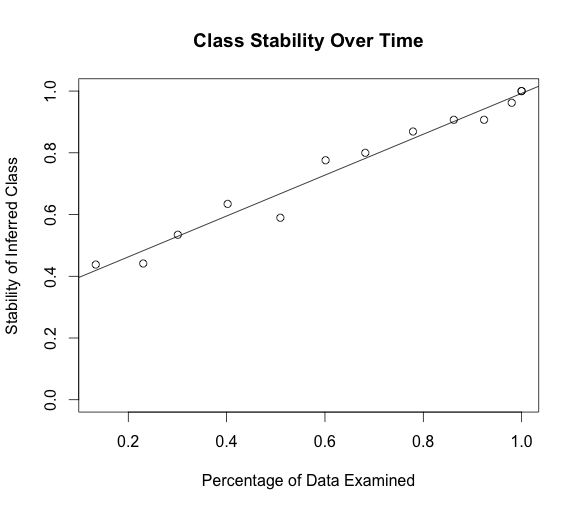
\includegraphics[scale=.4]{class-stability.png}
\caption{We measure the number of students who were classified into their ultimate strategy profile as the amount of data available to EM is increased. We see that at about 60\% of the data we can classify about 75\% of the students into their ultimate profile.}
\label{fig:class-stability}
\end{figure}

If an intelligent tutoring system could implement our classification methodology on-the-fly, it could tailor its pedagogical interventions to the needs of the individual student. To substantiate the promise of the methodology we investigate how efficiently the algorithm stabilizes to the final classification. To measure this, we first cluster on the entire corpus and assign each student to their most likely profile. We then artificially subset the data by restricting the number of problems seen by the clustering algorithm, compute the proportion of students who are in their ``final'' profile, and then iteratively increase the size of the subset. This simulates how well our algorithm identifies student profiles as they make their way through the material. 

% TODO FIXME wrt num problems
Figure \ref{fig:class-stability} shows the percentage of total data used to estimate the model plotted against the proportion of students assigned to their final strategy profile. At each iteration, we look at an additional 10 problems from each student and re-estimate the cluster assignments. The regression estimates that 63\% of the data is sufficient to classify three quarters of the students into their ultimate cluster. Thus, after seeing about 60 problems -- about two days of classroom instruction -- a dynamic intelligent tutoring system might intervene on students who fit the ``stubborn'' profile by ensuring that they are presented with multiple graphical representations, offering them spontaneous hints or targeting them with some other form of metacognitive support. 

\section{Conclusion \& Future Work}
\label{sec:conclusion}

We estimated a expectation maximization clustering model to classify students into four strategic profiles based on their error-rates and hint-seeking behaviors. We detected an affect of experimental condition on post-test outcome only in the class of students characterized by high-error rate and low hint-seeking propensity. That is, students who did not seem to take full advantage of the resources that the Mathtutor offered were the ones most strongly affected by experimental condition. These students may not have the meta-cognitive skills required to know when to seek hints. 

Our methods could be used by ITS designers to detect students with this profile in real time. Tutoring systems could then intervene to target these students with multiple representations, scaffold their hint-seeking behaviors or target them with other forms of metacognitive support. Future research into  the mediating mechanisms of multiple representations could leverage our results to identify the relevant student sub-populations to investigate. Our post-hoc analysis is not designed to identify the cognitive processes underlying the student's problem solving behavior, so interviews or a cognitive task analysis with students who fit the ``stubborn'' profile could reveal more details about their experience than we can detect from the log data. Additional investigation into different features may help further characterize student behavior and could help us more accurately group students into relevant subpopulations. Although our analysis seems to have revealed interesting differences in student learning strategies, more informative features constructed from log data may do better. Constructing more informative features, for example, might allow us to separate the ``stubborn'' students into those who did and did not benefit from multiple graphical representations. 

\bibliographystyle{abbrv}
\bibliography{references}

\balancecolumns
% That's all folks!
\end{document}
